
\section{Introduction}



Recently, large language models (LLMs) have excelled on diverse reasoning tasks via explicit chain-of-thought (CoT) rationales~\citep{wei2022chain,wang2022self,kojima2022large,qin2024large}. Yet, they struggle to cold-start from instruction-tuned or base models into Long CoT models requiring extended multi-step reasoning~\citep{chen2025towards,chen-etal-2025-unveiling-key}. Notably, \citet{du2025the} shows that humans generate Long CoT rationales without imitating DeepSeek-R1~\citep{guo2025deepseek}. Our preliminary studies reveal that standard supervised fine-tuning and distillation from human or Instruction LLM rationales (using randomly sampled Long CoT examples) fail to reliably instill these skills in LLMs. Models often lose coherence over long trajectories or fail to transfer patterns to novel tasks. This prompts a key question:

\begin{quotation}
{\begin{center}
    \textbf{How do Large Language Models learn and represent effective Long Chain-of-Thought?}
\end{center}}
\end{quotation}



\begin{figure*}[t]
    \centering
    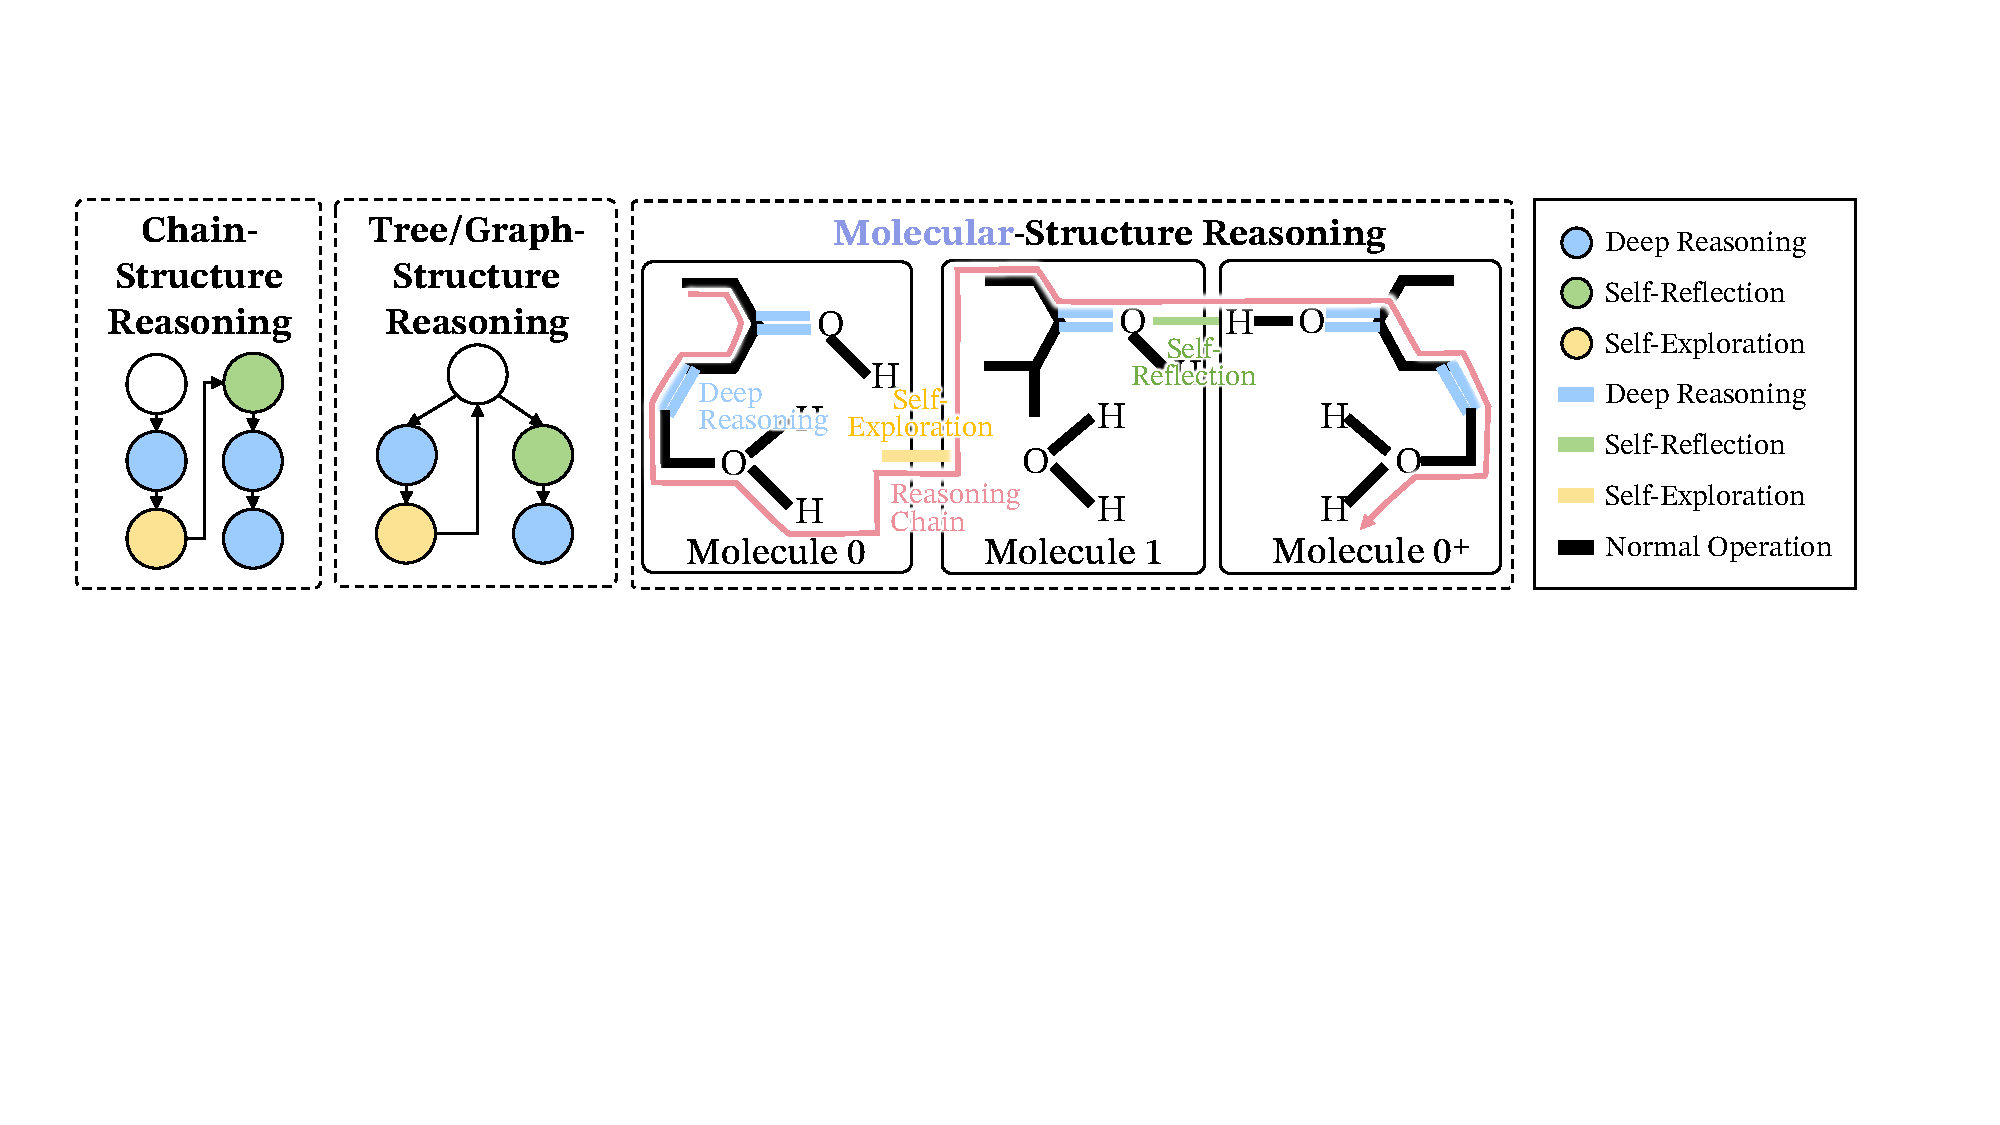
\includegraphics[width=0.98\textwidth]{figures/intro.pdf}
    \caption{Comparison of prior chain- or tree-like structures and our molecular structure. Reasoning starts from Mole. 0, uses \textbf{deep reasoning} on strongly related structures, then employs \textbf{self-exploration} for new logic in Mole. 1. When meet errors, reasoning utilize \textbf{self-reflection} to guide chain to optimized Mole. 0$^{+}$.}
    
    \label{fig:intro}
\end{figure*}


To explain this, we posit that they acquire the organization of reasoning trajectories. As shown in Figure~\ref{fig:intro}, prior studies model these as \emph{logic nodes} in sequences or trees of steps. Yet, our analysis of Long CoT across strong reasoning models reveals a stable distribution of three core behaviors across tasks and architectures: Deep-Reasoning, Self-Reflection, and Self-Exploration~\citep{chen2025towards}, which node-centric views fail to capture.



This finding triggers a molecular-inspired, distributional view: we model behavior-labeled \emph{logic edges} as interaction bonds and examine how their global \textbf{molecular-like structure} ensures long-horizon reasoning stability. Specifically, Deep-Reasoning forms dense local clusters of coupled deductions, like covalent bonds; Self-Reflection creates long-range corrective links to prior steps, like hydrogen bonds; and Self-Exploration forges weak bridges between distant clusters, like van der Waals forces. Thus, high-quality Long CoT arises from the {\textbf{stable composition and arrangement of these bond types}}, guiding effective learning\footnote{Note: C, H, and O atom references are analogies for molecular structure only.}.

In this framework, we define semantic isomers as Long CoT trajectories that solve the same tasks and visit similar semantic regions but differ in behavior distributions and transitions. We demonstrate that multiple near-optimal semantic isomers exist per task family, but mixing stable isomers from different strong teachers destabilizes learning, degrading performance and behavior distributions despite matched token statistics. This structurally explains why combining heterogeneous Long CoT traces often fails, beyond token-level distillation.



Building on this perspective, we propose \method, a structure-aware synthesis framework that first estimates a behavior transition graph from strong reasoning models and then transfers only this behavioral structure to cheaper instruction LLMs via controlled trajectory synthesis, instead of directly copying teacher outputs. This decouples structural transfer from model-specific surface form, enables the generation of Long CoT data that match target behavior distributions from scratch, and yields consistent gains in both Long CoT performance and RL stability across six  benchmarks.







After that, we analyze the shaping function of each bond in the Long CoT structure. Deep Reasoning bonds encode core logical flow, Self-Reflection bonds support folding pathways to previous steps, and Self-Exploration bonds reinforce long-range consistency checks, enabling targeted bond distributions. Moreover, we discuss why a deteriorated molecular structure is hard to restore, which helps explain how private LLMs protect Long CoT structures from distillation-based imitation. Methods such as summarization and reasoning compression can disrupt Long CoT structure, limiting unauthorized replication of internal reasoning processes.




In summary, our contributions are as follows:
\begin{itemize}[leftmargin=16pt, itemsep=0pt, topsep=0pt]
\item We model Long CoT as a molecular structure with 3 bonds: deep-reasoning (covalent), self-reflection (hydrogen-bond), and self-exploration (van der Waals), to understand its effective learning.
\item We identify effective Semantic Isomers for Long CoT learning, where only entropy-convergent bonds enable stable learning, while competing structures destabilize learning.
\item We introduce \method, which uses distribution-transfer graphs to synthesize these structures, improving Long CoT and stabilizing RL across 6 benchmarks.
\end{itemize}

